\chapter{Method} 

%The method chapter should describe in detail which activities you undertake to answer the research questions presented in the introduction, and why they were chosen. This includes detailed descriptions of experiments, surveys, computations, data analysis, statistical tests etc.

\section{Introduction}


As a background for the thesis, assume a threat actor is
 in a preliminary phase of an attack. The decision to initiate a phase of attack simulation is made, with the aim of gathering useful information in order to learn more about possible risks of being detected, as well as to gain some empirical background for the evaluation of possible consequences of a successful attack.
The potential outcome of the simulation may be used in order to prepare for attacking the actual infrastructure with attacks with a low attack detection probability and, to the best possible knowledge, with foreseeable consequences of the attack.

As described previously, the aim of the thesis is to investigate any observable effects of specific time delay attack simulations. Such simulations could be executed in a preparation phase, preparing for the execution of an actual time delay attack.

 \hl{Some papers} describes a number of varieties of the PTP delay attack, while \hl{other papers} describes the attack to have severe consequences to the \acrshort{sg} infrastructure. The primary goal of the actual attack is to stay undetected, while exposing the infrastructure under attack to an attack having the most severe consequences possible, while still avoiding detection.  
 


%For the \acrfull{wams} Security parts, a small number of surveys, as well as a collection of papers are investigated, covering  synchrophasor protocol attack vulnerabilities, highlithing some known side effects of successful synchrophasor protocol attacks. The introductory brief coverage of \acrshort{sg} security, is followed by a coverage of common synchrophasor protocols, focusing on attack vulnerabilities of the protocols covered. \\ 






%Several test cases utilising PMUs and PDCs



%In order to investigate, systems like mininet. \\ 


\section{Research Design}
%This section will inform the reader of the NATURE of your study. In other words, broadly speaking: are you aiming to describe a phenomena (descriptive design), are you aiming to explore a topic (exploratory design), are you looking to identify causal relationships between factors (causal design)?

%The aim of the thesis, is to present an overview of concepts, as well as to to provide examples from the literature related to the Smart Grid WAMS being vulnerable to attacks on the Synchrophasor protocols. 
In order to be able to observe the effects of exposing a \acrshort{pmu} to a time delay attack, the real attack is dependant on getting access to expensive equipment, like a \acrshort{pmu} as well as the interconnected infrastructure.
As previously discussed, a time delay attack on Synchrophasors imposes a high risk of causing damage to the infrastructure targeted.
Given the high potential for damage, a good option for visualising any potential effects a time delay might have on the values produced by a \acrshort{pmu} under attack, would be to simulate the attacks.
There exists a number of projects which utilises MATLAB and SIMULINK in order to model power grid components in general and, specifically, \acrshort{pmu}s.

My selected approach, however is to produce a SIMULINK model, using standard components from the Simscape Electrical addon to MATLAB/SIMULINK. The simulation produces pair-wise (original, delayed) PMU output values for each of the channels Magnitude, Angle and Frequency, making them available for comparison and further analysis. \hl{The analytic part could be one obvious candidate for further work.}

%
%Two identical copies of the PLL PMU is connected to a power source, one directly, the other via the delay function. The resulting output is pair-wise collected to one channel for each of the components Magnitude, frequenct

%In order to 

%Based on the findings of the initial literature study concerning vulnerabilities, the literature study continues providing potential scenarios for stealthy MiTM attacks on the synchrophasor transmission system, investigating the success of the attacks maximising side effects while minimising the probability of being detected.

As the final part of the thesis, a theoretical discussion, aiming to provide answers to the research questions, will be conducted.\\ 

%\textbf{TO DO:}
%\hl{As a experimental part of the thesis, possibilities of testing one or more detection and mitigation techniques might provide a contribution to the final discussion and conclusions based on my own experimental results}


\section{Research Methods}
As the thesis includes both a theoretical, as well as a more practical phase, the methods are dependant on the phase in question.
%Following the description of your research design, you should also devote a section to describing the research methods you applied during your study. Each design will provide you with many possibilities of methods to use.
\subsection{Theoretical phase}
As part of the introductory studies of the topic selected, a couple of searches on the NTNU literature search facilities returned a number of books, like \cite{BlumeStevenW2007Epsb} and \cite{kabalci2019smart}, covering introductory chapters on Power Grid and Smart Grid. The introductory chapters heavily relies on descriptions from relevant book chapters. 

\subsection{Practical phase}


In order to provide theoretical evidence on which to answer the research questions, a literature study will be conducted.
For any experimental results, experiments will be described, implemented and executed.

\section{Measurements}

%Once you clarified the method you used, it is time to explain exactly WHAT you measured (e.g. service quality, brand image, satisfaction, purchase intention) and HOW you measured

%Vulnerability to time-shift attacks are quantified by articles describing theoretical aspects of the mechanisms for the calculation of valid time-stamps, and the inherent tolerance level for calculation errors. 
%Modern Smart Grids require the time deviating from the correct time by a fraction of a millisecond. Specifically, according to \cite[p.  1953]{moussa2016security}, the allowed time deviation for a 50Hz electrical system\footnote{As used in Norway, for instance} must be within $\pm31.8\mu s$, in order to adhere to the 1$\%$ \acrfull{tve} requirement, as specified by the  IEEE C37.118 standard. \\ 


The simulations to be defined and executed provides examples of \acrlong{pmu} output, where two identical \acrshort{pmu}s are given a signal from a simulated power source as input. One of the PMUs are fed the original power source signal, whereas the other PMU is fed a delayed version of the original power source signal. The resulting PMU output measurements may be compared for similarity. 

Where possible, experimental investigations reported by articles selected will be provided as relevant examples, in order to support any discussion arguments for the purpose of reaching conclusions.  

\section{Sample}

%In this section you should detail (at least!) the population of your study, your sampling technique (which technique you used to select the people who took part in your study) and how you established your sample size.
The samples for my literature study will be papers relevant for the discussions, in order to provide answers to the research questions.\\ 

Any execution of experiments will provide experimental samples, with the aim of supporting discussions and conclusions.
The samples originating from the experiments, consists of:
\begin{itemize}
    \item Three channels of PMU output, denoted \textbf{Magnitude}, \textbf{Frequency} and \textbf{Angle} 
    \item Two arrays of numerical values for each channel of PMU output: One for the original signal, the other for the delayed signal. 
\end{itemize}
\section{Validity and Reliability}

%Now, here is a SUPER important section that 99\% get wrong(I completely made up this figure, simply because I want to convey a point!). Validity (that you measured what you intend to measure) and reliability (that the measurements used, such as your scales, are consistent and replicable) are two concepts that simply have to be addressed and have to do with your measurements.
In order to increase the validity and reliability, a number of articles will be included as the foundation for any conclusions. My personal selection of papers deemed relevant for my discussion, will be selected highlighting on articles being included as relevant articles by survey papers, as well as papers gaining a high relevance score on literature search sites.\footnote{... like the NTNU ORIA site (\url{https://innsida.ntnu.no/litteratur}).} Another selection criteria aiming to increase validity and reliability will be a focus on selecting articles receiving a high number of quotations ratings on sites like Google Scholar. %First and foremost, though, a sound and critical validation of the relevance for the questions at hand is still mandatory. \\  



For the experimental parts, my project is utilising a selection of PDC and PMU simulator packages. In order to validate the phasor data generated, the included validation capabilities of the simulator packages are utilised. 
\subsection{Validation of the model}
A experiment of running the simulation with a delay leve of 0, could serve two purposes:
\begin{itemize}
    \item Validation of the delay function
    \item Validation of the two copies of the PMU as being identical.
\end{itemize}
As a hyphothesis, running the simulation with a delay of zero should produce identical channel-wise output.

A $d=0$ test result  producing identical output for the who PMUs , would increase the 
confidence of the model both being valid and reliable.

Another criterion for a valid model would be for the data to show alterations which could be explained by a change of delay level.



\section{Infrastructure used during experiments }
%\hl{A selection of a relevant infrastructure for experiments will be made according to  specific needs and availability.  }\\ 

In order to provide practical results on which to base the discussions and conclusions, the following tools will be utilised;

\begin{itemize}
%    \item The iPMU suite, including iPDC, iPMU and PMUSimulator, running on virtual Ubuntu Linux instances
%    \item The pyPMU suite, including tinyPDC, tinyPMU and , running on virtual Ubuntu Linux instances \cite{vsandi2015python}, \cite{vsandi2016pypmu}
    %\item A SIMULINK model, downloaded from \textbf{URL} is used as the basis for the simulations.
    \item MATLAB, R2023a, with SIMULINK added, is used for running the simulation. 
    \item Simscape Electric, and its dependency Simscape, are required in order to build, and run, the simulations.
    \item The Simulation is executed by running a MATLAB script.
    \item A Windows 10 laptop is being used for the simulations
    
 %   \item mininet will be utilised for networking
 %   \item Wireshark will be utilised for synchrophasor packet analysis
 %   \item Python will be utilised in order to visualise the results

\end{itemize}

%\section{Instruments or Equipment}

%Sometimes, especially in causal studies when researchers are developing experiments, it is important to detail the instruments or equipment that were used in the study.



\section{Simulating a Time Delay attack}


\subsection{Scenarios}

For the experimental part of my thesis, a number of attack scenarios will be required. The aim is to investigate various attack vectors which might be used by a sophisticated man-on-the-side threat actor in order to execute an attack while staying undetected. 

\subsection{Assumptions} 

A number of assumptions is stated, in order to narrow the scope of the thesis:

\begin{itemize}
    
\item \textbf{Attacker Policy:}\\   A sophisticated threat actor would most likely want to avoid detection by anyone protecting the targeted infrastructure.
Therefore, executing an attack which may be detected should be avoided at all costs.
As a consequence, any decisions related to actually executing the attack should be as a result of promising results following a stealthiness assessment process. Simulations of possible effects could be part of the stealthiness assessment process. 

\item \textbf{Attack Prerequisites:}\\   A stealthy attack with small impact is preferred over an attack having more severe impacts, at a higher risk of detection.
The ideal attack would be an attack having maximal impact on the target, while the risk of detection being minimal. 


\item \textbf{Attack Design Policy:}\\   A part of the challenge would be to design an attack producing a high impact on the target, while staying undetected.
\end{itemize}
\subsection{Approach Selected for the Attack:}
%One possible solution could be to determine the minimal efforts needed in order to execute an attack with a high probability of producing the effects desired, while keeping the attack detection probability low.


Consider targeting a system able to detect PMU output deviations exceeding a specified threshold. The detection system may classify a suspicious PMU output pattern as one of four categories, analogous to the classification categories described in \cite[p. 5]{kunang2021attack}: 
\begin{itemize}
    \item \acrfull{tp}: Output pattern correctly classified as an attack.
    \item \acrfull{tn}:  Output pattern correctly classified as no attack.
    \item \acrfull{fp}: Output pattern incorrectly classified as an attack.
    \item \acrfull{fn}: Output pattern incorrectly classified as no attack.

\end{itemize}

 
A viable strategy could be to focus on a few optional tolerance levels. Even without knowing the detection threshold of the system targeted, the attacker could benefit from being able to predict any consequences of a future attack. Three levels of tolerance could cover three potential scenarios:
\begin{enumerate}
    \item A tolerance level of 1\% may impose a high attack detection risk before the attacker is able to do much harm.
    \item A tolerance level of 5\% may impose a lower detection risk, enabling the attacker to do more harm
\label{item:i2}    \item A tolerance level of 10\% will impose an even lower detection risk, enabling the attacker to do even more harm, than in the previous case (Item \ref{item:i2}.).
    
\end{enumerate}

It may also be a good approach to determine any effects of a small increase in delay level, versus executing the attack using a fixed delay level.
%\begin{itemize}
%    \item Use the lowermost drawings appearing in each component output generated for graph comparisons.
%    \item Visually inspect the drawing for any red portions, indicating difference beyond the specified tolerance  level, indicating risk of attack detection.
%    \item The graphs may provide indications on attack stealthiness, by no, (or minimal) red portions in the lower drawing. 
%    \item Tolerance levels: $1\% (0.01)$, $5\% (0.05)$ and $10\% (0.1)$.
%\end{itemize}

%\begin{enumerate}
%    \item The green portion of the line indicates signal similarity, indication periods with a low probability of attack detection.
%    \item The red portion of the graph is to be interpreted as time periods where the attack detection risk is too high for the attack to remain stealthy for lengthy periods of time.

%\end{enumerate}



\subsection{Attack scenarios}
In order to provide experimental results in order to answer the Research Questions stated, a number of attack scenarios are defined.
The main method of simulation would be a delayed forwarding of values, where a specified number of delayed samples, $d$, is applied to the PMU input. The value of $d$ is used to replace any sample $s(i)$ with the sample value $s(i-d)$, simulating\footnote{A specific SIMULINK delay module is performing the simulated delay of samples.} clock drift, producing effects similar to a \acrlong{tda}.
The simulation could be performed using a number of delay functions. For the thesis, two types of approaches are used:
\begin{itemize}
    \item The \textbf{Instant Delay Attack}, Increases the delay level to the targeted level at attack initiation. The attack maintains a constant delay level for the entire duration of the attack. 
    \item The \textbf{Step-wise Delay attack}, increasing the delay level by one sample each second, until the targeted delay level is reached. The attack maintains a constant delay level for the remaining duration of the attack.
\end{itemize}


\subsubsection{Attack characteristics}
In order to investigate some specific effects of the attack, the following characteristics are selected:

\begin{enumerate}
\item In order for the model to stabilise\footnote{The PMU needs some samples of input before being able to stabilise the output values.}, data used for visualisation does not include the first second of the simulation ($t < 1$).
\item In order to be able to conclude on the effect of delay cancellation, knowledge of the system state prior to the attack is required. Therefore, each simulation is executed  with a delay level of 0 for the next second ($1 < t < 2$). 
\item  The Instant Delay Attack involves raising the delay level instantly to a level $d > 0,  d \in \mathbb{N}$, at the time $t = 2$.
\item  The Step-Wise Delay Attack involves raising the delay level in steps of one each second, from $t = 2$ until reaching the level $d$ at $t = 1+d$.  
\item  In order to be able investigate any effects of attack cancellations, the targeted PMU is exposed to a delay attack for a limited time, thus reducing the delay level $d$ to $0$ before reaching the last second of the pre-set simulation running time.   
\end{enumerate}
    
 \begin{figure}[ht]
 \begin{center}
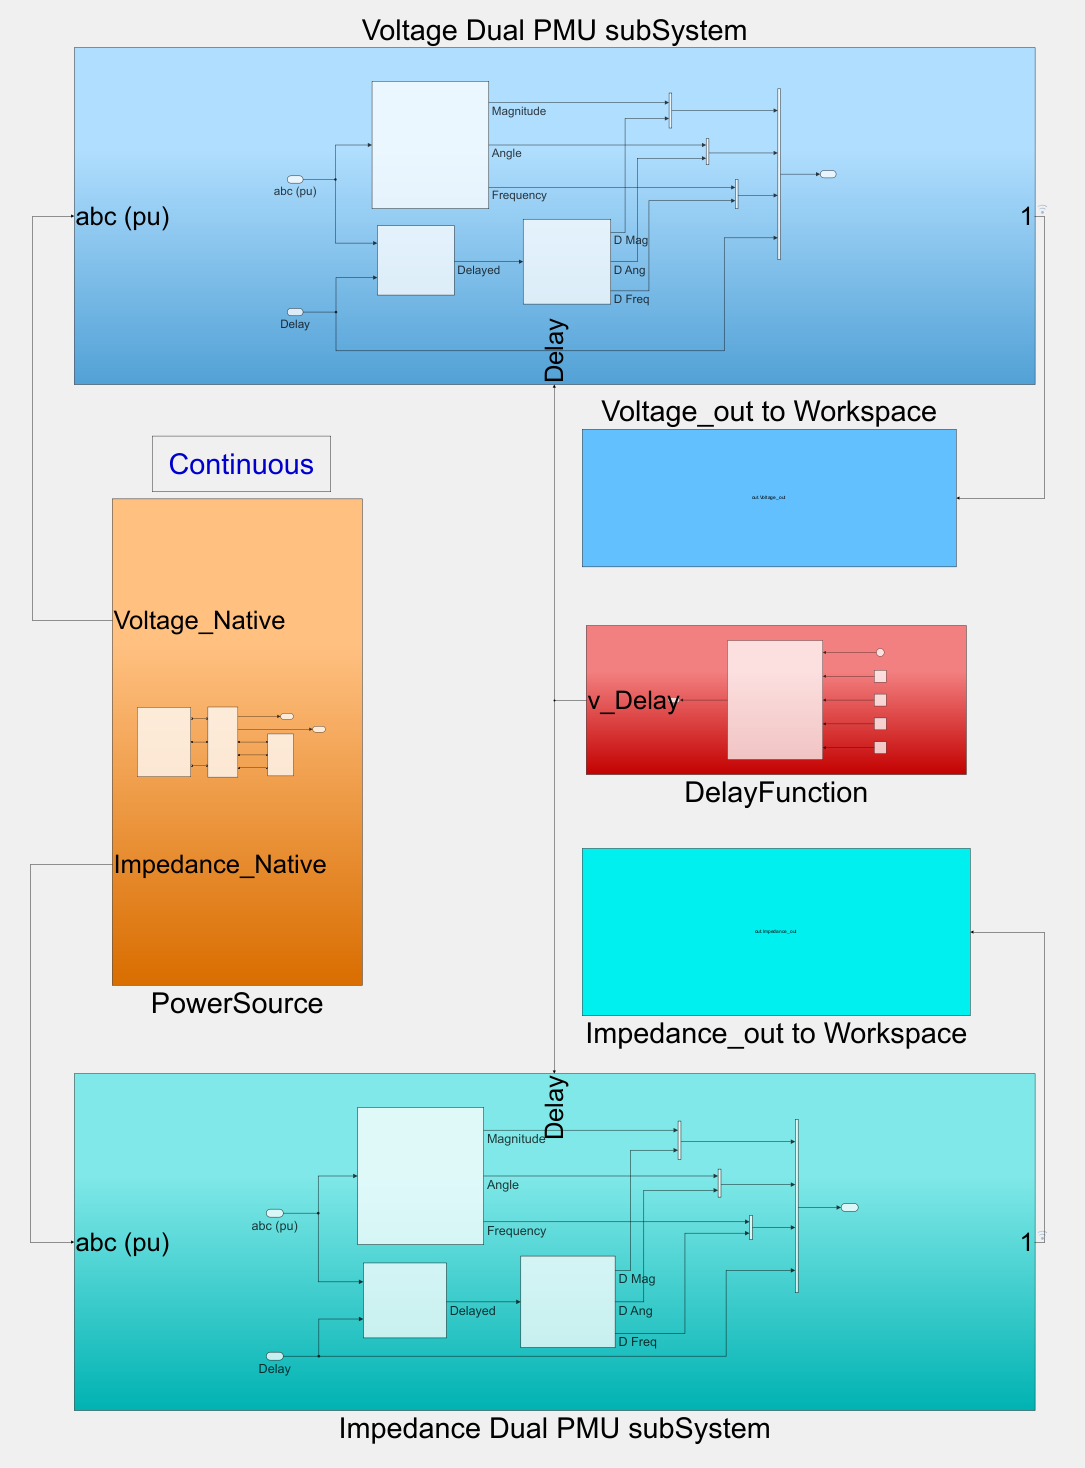
\includegraphics[width=0.9\textwidth]{figures/pmuSIM-overview.png}
\caption[PmuSIM SIMULINK model]{A SIMULINK model for the simulation of PMU Time Delay Attacks.}
\label{fig:PMUsim-Overview}
     
 \end{center}
\end{figure}


\subsection{Attack Simulation Implementation}
%The attacks would be implemented as MATLAB functions executing attacks on targets implemented as SIMULINK simulations. The various scenarios would  be required to be sufficiently similar to be implemented as variations of a single attack framework, in order to avoid the need of creating more than a single attack framework.     

%In order to prepare for attacks, a plan might be to implement the techniques described in \cite{gilad2014off}.



%\textbf{\cite{barreto2016undetectable} proves the requirement of exposing more than two PMUs to a delay attack, for the attack to be undetectable.}




A number of physical investigations related to the effects of any attacks on the intended targets, would increase the knowledge of a potentially complex target, increasing the probability of staying undetected during the attack. As previously explained, those investigations will be done in a simulation environment.
%In order to avoid exposing expensive and critical power system infrastructure to physical damage or downtime,\footnote{In a test lab environment, downtime could be acceptable, whereas the risk of physical damage of typically expensive equipment may be too high, at least not in the initial phases of investigations.} such practical investigations would preferably be performed in a simulation environment.

\section{Creating a Simulation environment}

%This approach could be taken by a threat actor during a phase of investigations in the preparation of the actual attack, for the purpose of learning more about the possible consequences of performing intended actions on the intended target. One of the most important priorities of the threat actor, is to stay undetected for as long as possible. 
Simulations are designed, in order to investigate the attack scenarios previously described. The planned attack is implemented using a combination of Simulink and MATLAB. The simulation produces three pairs of PMU channel output, one pair for each of the \textbf{Magnitude}, \textbf{Angle} and \textbf{Frequency} channels.
Each pair consists of the native\footnote{Native PMU output equals the PMU output with no input delay.} and delayed  PMU output signals. 

The execution of each simulation will, after the completion of the execution of the SIMULINK model, produce corresponding graphical output, included in the thesis as figures. The graphical representations are used to illustrate any visible effects the attack may have on the system. The graphs enable visual pair-wise comparison of the output produced by the attack. In addition, the graphical result of a numerical check for tolerance compliance is presented for visual inspection.

A PMU may include output channels for both Voltage and Impedance PMU input. The simulation covers both Voltage and Impedance pMU input.

\subsection{Modelling a PMU}

As the plan of the threat actor is to expose  a number of \acrshort{pmu}s to a time  delay attack, the plan is to build a model of a \acrshort{pmu}, allowing the model to be run for both Instant and Step-Wise attacks involving various time delay levels, in order to investigate any observable effects on the output from the \acrshort{pmu}.
\subsection{Model Description}
The SIMULINK model implemented consists of two SIMULINK Subsystems:
\begin{itemize}
    \item The \textbf{PowerSource} Subsystem, consists of a number of SimScape Electric components, producing simulated three-phase signals for both  Voltage and Impedance.
    \item \textbf{The DualPMU} Subsystem, accepts a simulated three-phase power input, and a delay level, and produces a six-channel signal for external processing. 
\end{itemize}


The model, shown in figure \ref{fig:PMUsim-Overview}, consists of one PowerSource Subsystem, connected to two DualPMU subsystems, one for each of the Voltage and Impedance PowerSource outputs.

\subsubsection{The PowerSource subsystem}


The main components of the sub system is available from the component libraries of the Simscape Electic addition to the SIMULINK/MATLAB software suite.

\begin{itemize}
    \item \textbf{Three-Phase source} 
    \item \textbf{Three-Phase V-I Measurement}  Providing Voltage and Impedance levels.
    \item \textbf{Three-Phase Parallel RLC Load}. Documentation at \cite{mathworksImplementThreephase}. 
\end{itemize}
In addition, two signals are provided as output from the subsystem to be used as PMU inputs:
\begin{enumerate}
    \item \textbf{Voltage\_ Native}: The non-delayed voltage signal.
    \item \textbf{Impedance\_Native}: The non-delayed Impedance signal.
\end{enumerate}

 \begin{figure}
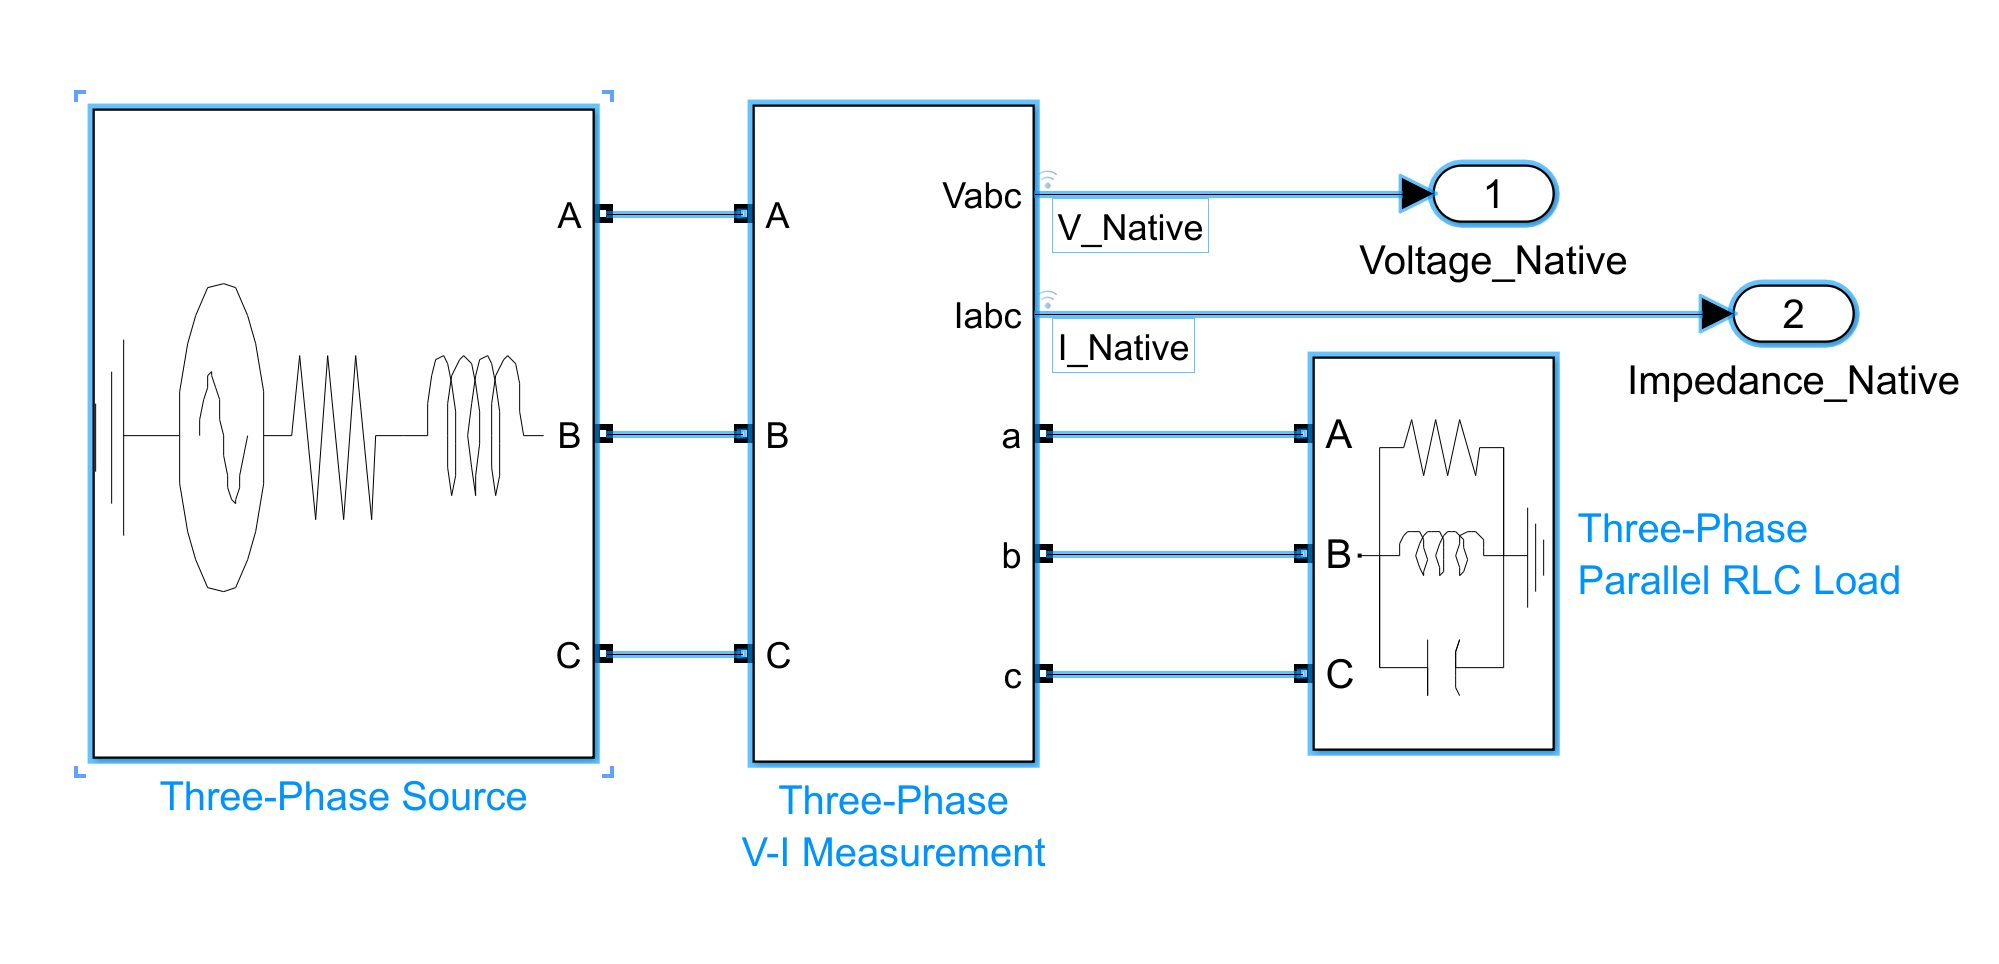
\includegraphics[width=0.9\textwidth]{figures/PowerSourceSubsystem.png}
\caption[PowerSource SIMULINK subsystem]{PowerSource: Generating  V and I PMU Input to DualPMU.}
\label{fig:PowerSource}
\end{figure}
  \begin{figure}
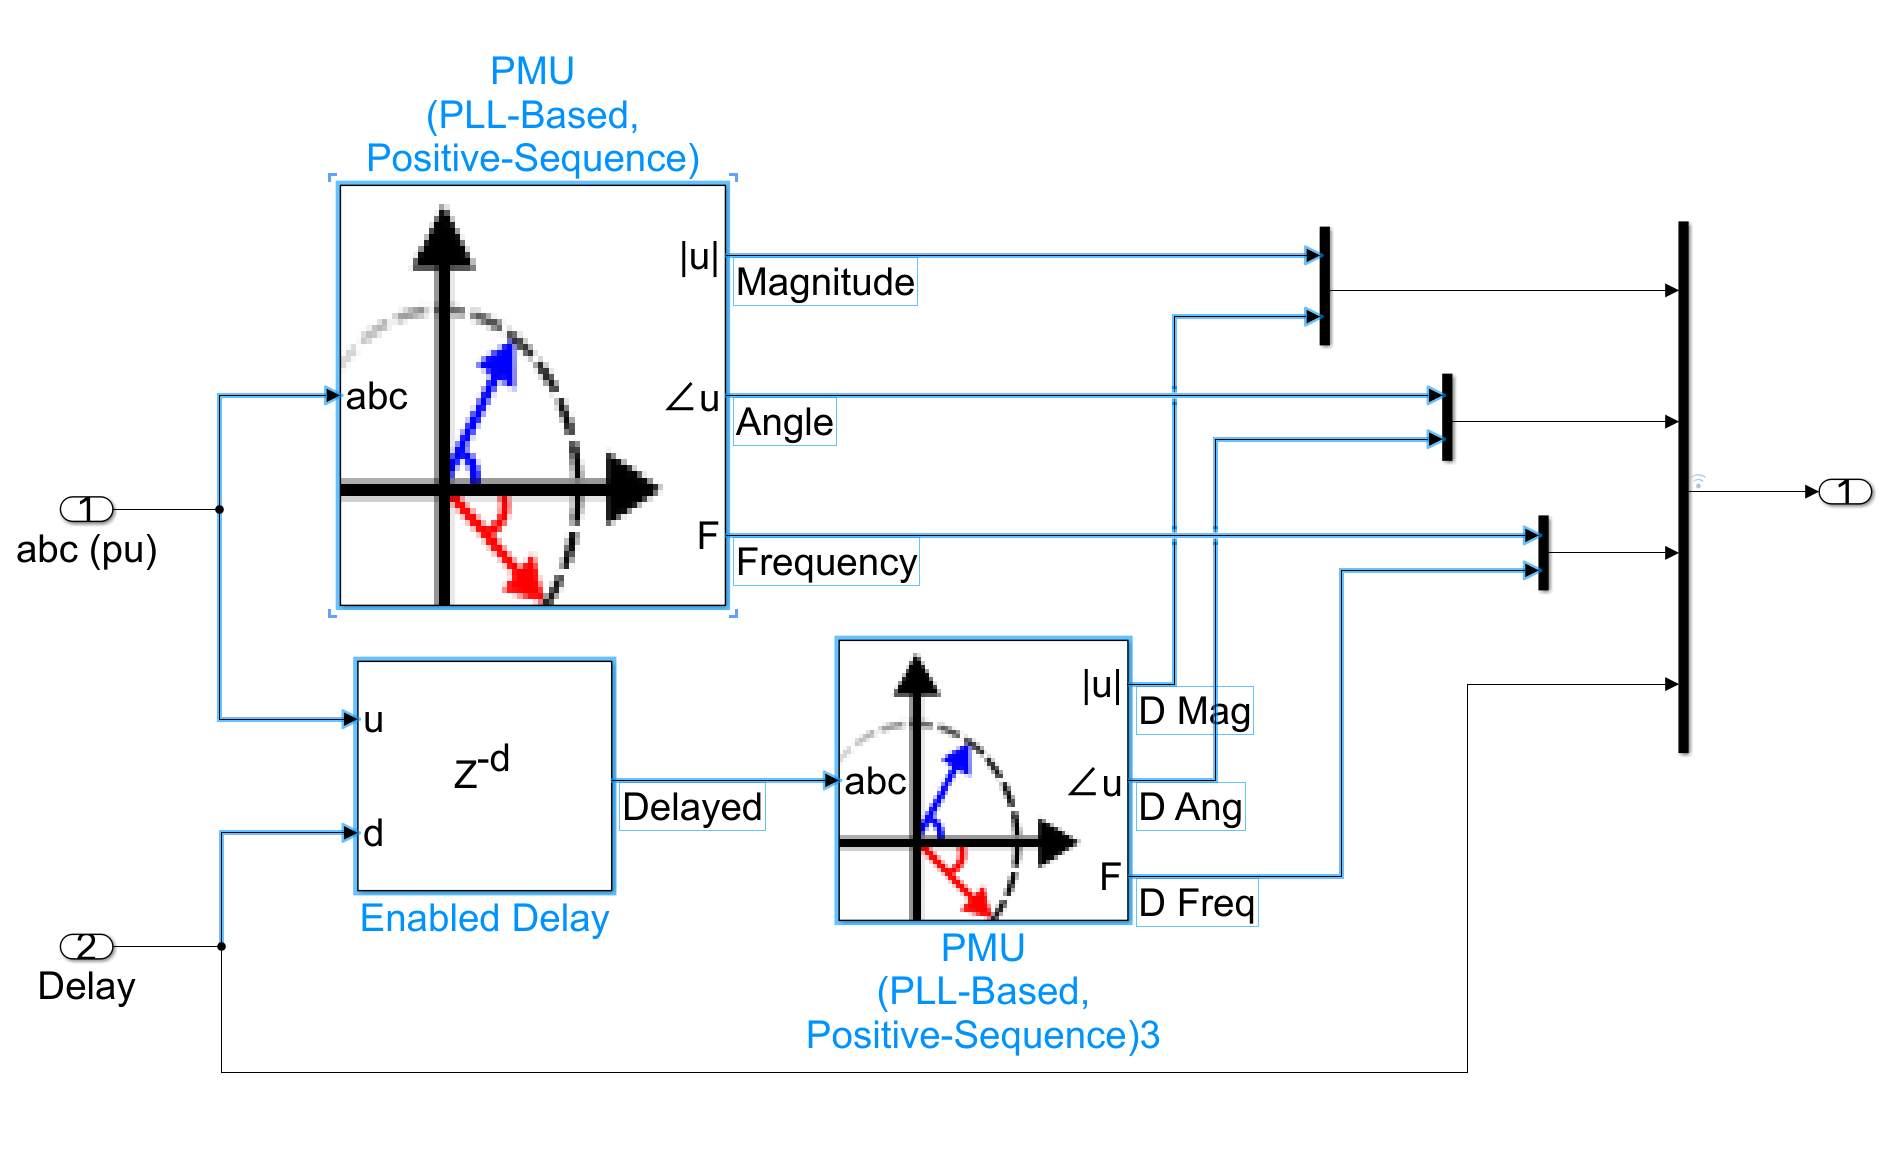
\includegraphics[width=0.9\textwidth]{figures/DualPMUsubsystem.png}
\caption[DualPMU SIMULINK subsystem]{DualPMU: Generating PMU output from V or I from PowerSource.}
\label{fig:DualPMU}
\end{figure}

The composition of the PowerSource Subsytem is visualised in figure \ref{fig:PowerSource}.

\newpage
\subsubsection{The DualPMU subsystem}
The composition of the DualPMU Subsytem is visualised in figure \ref{fig:DualPMU}.

The DualPMU subsystem consists of the following components:
\begin{itemize}
    \item A three-phase input, as provided by the Voltage or, alternatively, Impedance output of the PowerSource subsystem previously described.
    \item A numeric integer input, representing the delay level by which to 
    \item A \textbf{Delay} SIMULINK block, which produces a delayed signal from the PowerSystem Output, delayed by the value \textbf{d}, received at DualPMU Delay input from the DualPMU delay input port.
    \item Two identical PMUs are part of the DualPMU system: One accepting the original PMU input signal, the other accepting the delayed pMU input signal.
    \item Three 2to1 MUxes, collecting one PMU channel output pair each.
    \item One 4to1  MUX, collecting the combined PMU outputs from the three 2to1 muxes, one for each of the channels Magnitude, Frequency and Angle. 
    \item The fourth MUX input is connected to the unmodified delay input, in order to store the corresponding delay function for each simulation session, enabling its inclusion in the figures.
\end{itemize}

In addition to the PowerSource and the DualPMU subsystems, there are also some additional components included in the SIMULINK Model:
\begin{itemize}
    \item The Delay function, is implemented as a MATLAB function, which calculates the step-wise delay level, in addition to setting the constant delay level for the ouput, according to the rules for delay initiation and termination.
    \item Two SIMULINK blocs of type \textbf{to Workspace}:
    \begin{itemize}
        \item \textbf{Voltage\_out} storing the output from the Voltage DualPMU subsystem to a MATLAB workspace variable, for further processing.
        \item \textbf{Impedance\_out} storing the output from the Impedance DualPMU subsystem to a MATLAB workspace variable, for further processing.
    \end{itemize}

\end{itemize}

\subsection{Experimental Procedure}
%\textbf{TO DO:} \textit{Describe experimental procedure, dependant on experiments and experimental environment selected.}.
In order to execute the simulation, each step should be completed, as required.
\begin{enumerate}
    \item Start Matlab
    \item Open a MATLAB script, named \textbf{PMUsimScript.m}.
    \item Inspect and modify a selection of variables, and execute the script for each run. The script will produce:
    \begin{enumerate}
    \item Output data logged to workspace for each of the DualPMU subsystems voltage(V) and Impedance(I), to be further processed by the script at the end of each execution of the SIMULINK model.
    \item For each variation of PMU type (V/I), and channel (Magnitude/Angle/Frequency), a numeric comparison is followed by a corresponding colored (Red) similarity classification.
    \item One figure for each channel,  PMU type,  Delay function type, and Delay Level, is produced.
    \item Each figure is showing, for the specific configuration, a combined plot of the original and delayed signals. A number of plots, one for each of the tolerance levels of 0.01 (1\%), 0.05 (5\%), and 0.1 (10\%), is included in the same figure.
    \item The tolerance plots, shows  tolerance compliance information for a level, as well as a visualisation of the Delay function, and the normalised ([0,1]) difference between the native and delayed signals, for the signals in the plot above.
    \item Failure to comply to the tolerance level is visualised as red portions on the time scale.
    \end{enumerate}
    \item During script execution, each figure is displayed on screen for visual inspection, before being automatically saved at a specified location. 
\end{enumerate}
\subsection{Definition of Experiments} \label{sec:ExpDef}

%As discussed in an \textbf{Earlier Chapter}, according to \textbf{SELECTED PAPERS}, the \acrshort{sg} \acrshort{se} systems analysed would detect attacks producing signal differences of various levels of similarity. %around $10-15\%$ similarity.





The experiments will focus on various levels of assumed detection thresholds.

%My experiments will cover a selection of attack strategies for the selection of threshold levels of $1\%$, $5\%$ and $10\%$ similarities.

\begin{enumerate}
    \item \textbf{Immediate delay} Square pulse signal: Starting off, turning constant-delay on,  before dropping to 0 before simulation end. 
    \item \textbf{Step-wise delay} Increasing to delay level specified, in step-wise increase of delay level by one each second, before dropping to 0 before simulation end. 
    %\item Increasing delay, drop to 0 before simulation end
\end{enumerate}

Additionally, the  \textbf{No delay (, no\footnote{At least, if considering the attack with No Delay an attack, it will be pretty harmless. }) Attack}, running the simulation on a constant delay level of $0$ for the entire duration of the simulation, will be executed in order to produce output for model validation purposes. 

%\hl{The simulations need re-run}
%The current figures of chapter \ref{chap:Results} are produced by exposing the PMU to a variety of \textbf{d\_mode}s, as well as a selection of delay levels.



%The experiments, therefore, will focus on levels of delay of 0.1 to 0.15. For each level, the analysis will focus on various attack strategies, reaching the delay level in 1,2,3 and 4 steps, before keeping the delay for a total duration of  5 to 15 seconds.

%The experiments will be performed utilising \acrshort{pmu} simulation software, utilising available verification tools to ensure the compliance with established standards like the <--->
%The plan is to recreate experiments performed by <----> in a live environment, utilising  In order to test mitigation, mininet will be utilised

%Generate PMU data utilising simulators verified for compliance


%Utilise SADF \cite{SADF-framework} in MATLAB.

%Once again, in case you are running a causal study and an experiment, it is important to detail the experimental procedure.

%Explain, to the reader for example, what was the experimental task (what did the participants have to do?), the extraneous variables that were controlled (variables of the environment that could affect the cause and affect relationship).


